\documentclass[conference]{IEEEtran}
\usepackage[T1]{fontenc}
\usepackage[utf8]{inputenc}
\usepackage{graphicx,booktabs,amsmath,amssymb,url}
\title{Large-Scale Cyberattack Detection and Evolving Attack Pattern Mining: A Leakage-Aware Evaluation of Generalization, Drift and Adaptive Learning}
\author{\IEEEauthorblockN{[EDIT STUDENT NAME]}\IEEEauthorblockA{[EDIT DEPARTMENT AND INSTITUTION]\\{}[EDIT CITY, COUNTRY AND EMAIL]}}
\begin{document}\maketitle
\begin{abstract}This project evaluates leakage-aware cyberattack detection and evolving traffic patterns on a 16,232,943-flow source release and a 2,830,743-flow external mirror. Spark engineering, supervised and novelty models, open-set diagnostics, frequent patterns, historical drift, delayed-label adaptation and explainable inference are assessed with versioned evidence. Strong grouped-random results coexist with weak chronological recall; hybrid and adaptive policies show mixed trade-offs. External evaluation uses three conditionally compatible predictors and preserves source-only versus target-trained distinctions. Forty-eight volume/worker measurements, 16 warm-ups and 130 optimization measurements show workload-dependent performance: at one million matched rows, Pandas takes 0.242 seconds versus Spark 0.616 seconds for the measured query. A separate dashboard executes archived LR, RF and K-Means with 2,445 Spark parity probes. The contribution is an auditable experimental and software chain, not a production detector or a state-of-the-art claim.\end{abstract}
\begin{IEEEkeywords}intrusion detection, leakage-aware evaluation, Spark, drift, adaptive learning\end{IEEEkeywords}
\section{Introduction}
Network intrusion research often reports high held-out accuracy without asking whether the evaluation resembles future captures. This project treats data provenance, split design and operating thresholds as part of the scientific problem. It studies the exact MMDS Kaggle release and a separately documented CICIDS2017 mirror, preserving original population counts and the uncertainty of their upstream extraction chains.

The work combines Spark engineering, supervised and novelty models, family rejection, pattern mining, retrospective drift analysis, delayed-label adaptive policies and a validated demonstration application. Its central result is not that a complex detector solves cyberattack detection. It is that numerical correctness, random-split ranking, future operating-point recall and deployable model compatibility are distinct claims that require different evidence.

The report follows that distinction throughout. The source corpus contains 16,232,943 flows; purged chronological test cohorts, the 15,322,987-flow historical replay, the 1,997,636-row adaptive primary evaluation and the 308,939-row primary external test are not interchangeable denominators. All comparisons retain their declared feature sets, training budgets, calibration rules and label availability.

Given a heterogeneous historical flow corpus, construct reproducible numerical layers and evaluate whether detectors trained on earlier or grouped observations maintain useful attack recall at a defensible benign false-positive burden. Extend the analysis to unfamiliar families and external data without assuming that similar column names imply identical measurement semantics.

A second problem is engineering assurance: every displayed result should be traceable to a versioned input, model, transform, threshold and evaluation denominator. A third is computational: measure actual workload actions under a constrained single-machine Spark environment, separating data-volume, thread, storage and cache effects from unsupported multi-node or production claims.

Correlated duplicate flows can make a row-random split unrealistically easy. Class imbalance can make majority predictions look accurate, while a model with useful ranking can still miss almost every attack at its operational threshold. Marginal distribution alarms can also reflect capture composition rather than a changed decision boundary. These failure modes motivate a study that retains negative findings and unsupported claims instead of selecting only a favorable result.

The academic motivation is to connect algorithms with experimental discipline. The engineering motivation is to provide auditable artifacts and a usable demonstration that computes real predictions rather than replaying static labels. The project does not promise a live network sensor, autonomous defense or a production security service.

\section{Related Work}
Spark supplies a unified processing model and MLlib provides reusable learning pipelines \cite{spark,mllib}. Random forests and gradient boosting are established ensemble methods \cite{forest,boosting}; neither algorithm's reputation guarantees performance on a temporally different flow population. FP-growth supplies a compact frequency-mining strategy \cite{fpgrowth}. The present project uses these algorithms as reproducible components, not as newly invented methods.

ADWIN and concept-drift literature motivate explicit change-monitoring assumptions \cite{adwin,drift}. Controlled synthetic episode labels allow delay and stationary-alarm evaluation, whereas the historical captures have no authoritative concept-drift ground truth. Precisionrecall analysis is relevant under class imbalance \cite{pr}, but the study reports both ranking and frozen-threshold decisions rather than treating one curve as sufficient.

SHAP gives an additive attribution framework \cite{shap}. Here exact interventional linear contributions are validated in log-odds, while unsupported direct tree explanations are omitted. TESSERACT studies spatial and temporal evaluation bias in malware classification \cite{tesseract}; it motivates caution about experiment design but is not an intrusion-detection baseline or a quantitative comparator for these flow results.

CICIDS2017 is documented by its dataset paper and institutional release \cite{cicids,unb}. The accessible Kaggle mirror is version-pinned and audited, while byte identity to an official archive and exact extractor builds remain unverified. Related work therefore informs methodology and terminology; this report makes no state-of-the-art comparison or publication-acceptance claim.

\section{Research Contributions}
The first contribution is an auditable data and evaluation chain across the exact 16,232,943-flow source release, with predictor-equivalence role separation, training-only transforms and retained denominators. The second is a coherent negative-result account of temporal/family generalization, calibration, novelty, fusion and delayed-label adaptation.

The third contribution is model-level numerical assurance: exact LR logits, centroid distance, hybrid paths, validated linear SHAP and portable LR/RF/K-Means execution have explicit reconstruction or parity checks. The fourth is a matched computational study that forces consumed numeric/model outputs and distinguishes workload scale, threads, format and cache. The fifth is a demonstration-ready research application and an academic package whose figures, tables and claims are content-addressed.

These contributions are supported within this project. There is no claimed new classifier, benchmark superiority, causal attack discovery, prospective live defense validation or multi-node scaling theorem.

\section{Methodology}
The system separates private data engineering, scientific evaluation and public demonstration artifacts. Private Kaggle CPU jobs verify pinned inputs and persist fitted pipelines plus compact aggregate receipts. Independent verification checks numerical reconstructions, calibration, model components and scope counts. Git stores approved aggregates, source/configuration, model identities and bounded portable parameters, not raw private flow records.

The advanced application reads immutable evidence and verifies its own model artifacts before computing manual or bounded CSV predictions. It does not call Kaggle or fit preprocessing on uploaded values. The academic submission reuses those accepted outputs and adds only conceptual architecture diagrams, editorial synthesis and document-quality verification.

The end-to-end architecture has six boundaries: input provenance, audited numerical representation, experimental role assignment, fitted/scored research components, immutable evidence/model registries and consumer-facing artifacts. Each boundary has an explicit contract. This is important because a correct classifier can still be evaluated on the wrong population, and a correct table can still be mislabeled in a dashboard.

Training-only transforms and frozen operating thresholds constrain information flow. Historical replay preserves archived order without implying live monitoring. Adaptive candidates become active only in a future window after allowed labels and calibration are available. Portable inference preserves original parameters but does not create a new empirical generalization claim.

The objectives are: audit the exact released population; create reusable typed and finite Spark layers; separate grouped-random, chronological and holdout performance; evaluate reference novelty and hybrid policies on matched cohorts; distinguish family-stage diagnostics from upstream binary misses; mine frequent and emerging associations with explicit supports; study historical signals and controlled synthetic changes separately; enforce predict-before-label-release adaptation; reconstruct supported explanations; evaluate conditional common-feature external models; measure bounded scalability workloads; and expose verified archived inference in an isolated application.

Success is defined by reproducible evidence and completed acceptance gates, not a minimum accuracy chosen after observing results. An unsupported feature contract, undefined metric or failed engineering version is recorded explicitly. Public deployment and prospective effectiveness are outside the completed experimental scope.

\section{Experimental Design}
The project addresses a reproducibility gap between a favorable model score and the evidence needed to interpret it. The relevant gaps are incomplete cohort accounting, leakage through repeated predictor vectors, unseparated threshold effects, unsupported feature harmonization, retrospective labels described as online learning, attribution without reconstruction checks, and performance claims based on unconsumed lazy actions.

The contribution is an integrated, traceable case study across these concerns. It does not claim to be the first use of Spark, random forests, drift detection or explainable intrusion analysis. The strongest supported novelty is project-level experimental integration and transparent negative-result evidence, not a new learning-theoretic algorithm.

\subsection{Population and representation contracts}
The source release contains 16,232,943 flows, including 13,484,708 benign and 2,748,235 attack rows. Fourteen capture-only timestamp flags yield a different strict population of 16,232,929; this is not a second estimate of the same inclusion rule. Typed numerical features are audited for finite values, malformed inputs and zero denominators. Learned imputation, signed logarithms where specified, centering, scaling and estimators are fitted on training roles only. The full archived inference contract uses 18 ordered features; the separate external experiment retrains conditional common-feature baselines with only three features. These models must not be described as the same transfer experiment.

Protocol A uses grouped-random roles; B uses chronological capture roles with cross-role duplicate purging; C evaluates an unseen-family setting. Their final train/validation/test populations are respectively 11,455,925/2,344,726/2,432,292; 13,191,622/1,151,256/980,109; and 13,522,722/392,902/1,458,218. Purged counts are zero, 909,956 and 859,101. The retained B-role union is 15,322,987 and supplies a 49-batch historical replay. Training samples are independently reported rather than mislabeled as the full training population.

\subsection{Scores, decisions and comparison units}
For a threshold $\tau$, $\hat y=\mathbb{1}[s(x)\geq\tau]$, recall is $TP/(TP+FN)$ and the benign false-positive rate is $FP/(FP+TN)$. Undefined denominators remain undefined. A model's precision--recall curve summarizes ranking across thresholds; it does not establish usefulness at a frozen operating point. Thresholds are selected on validation roles and then frozen. Target-test labels are not used to tune external decisions. K-Means distance and hybrid novelty scores are not calibrated attack probabilities.

The external AUC implementation uses 2,048 bins, a step precision--recall integral and trapezoidal ROC integral. These are documented approximations, not exact continuous-score integrals. Comparing these values with unrelated implementations requires checking tie handling and binning. Neither accuracy nor an isolated AUC replaces the reported class counts and operating-point errors.

\subsection{Temporal patterns, drift and adaptation}
FP-growth mines six discretized feature items per flow, and association rules express conditional support and confidence rather than causal influence. Support sensitivity is evaluated at fixed full-source population. Emerging patterns compare declared captures; capture composition and attack prevalence can confound apparent emergence. Historical observations are distinguished from controlled synthetic changes, for which episode targets permit detection and delay accounting.

Adaptive replay predicts before labels are released. Delayed labels enter only the permitted update window; calibration and candidate promotion follow the declared policy. A candidate trained in a window cannot retroactively change that window's predictions. Cooldown, training budgets, rolling history and incumbent retention are explicit constraints. This simulated availability protocol is scientifically narrower than prospective online adaptation.

\begin{figure}[t]\centering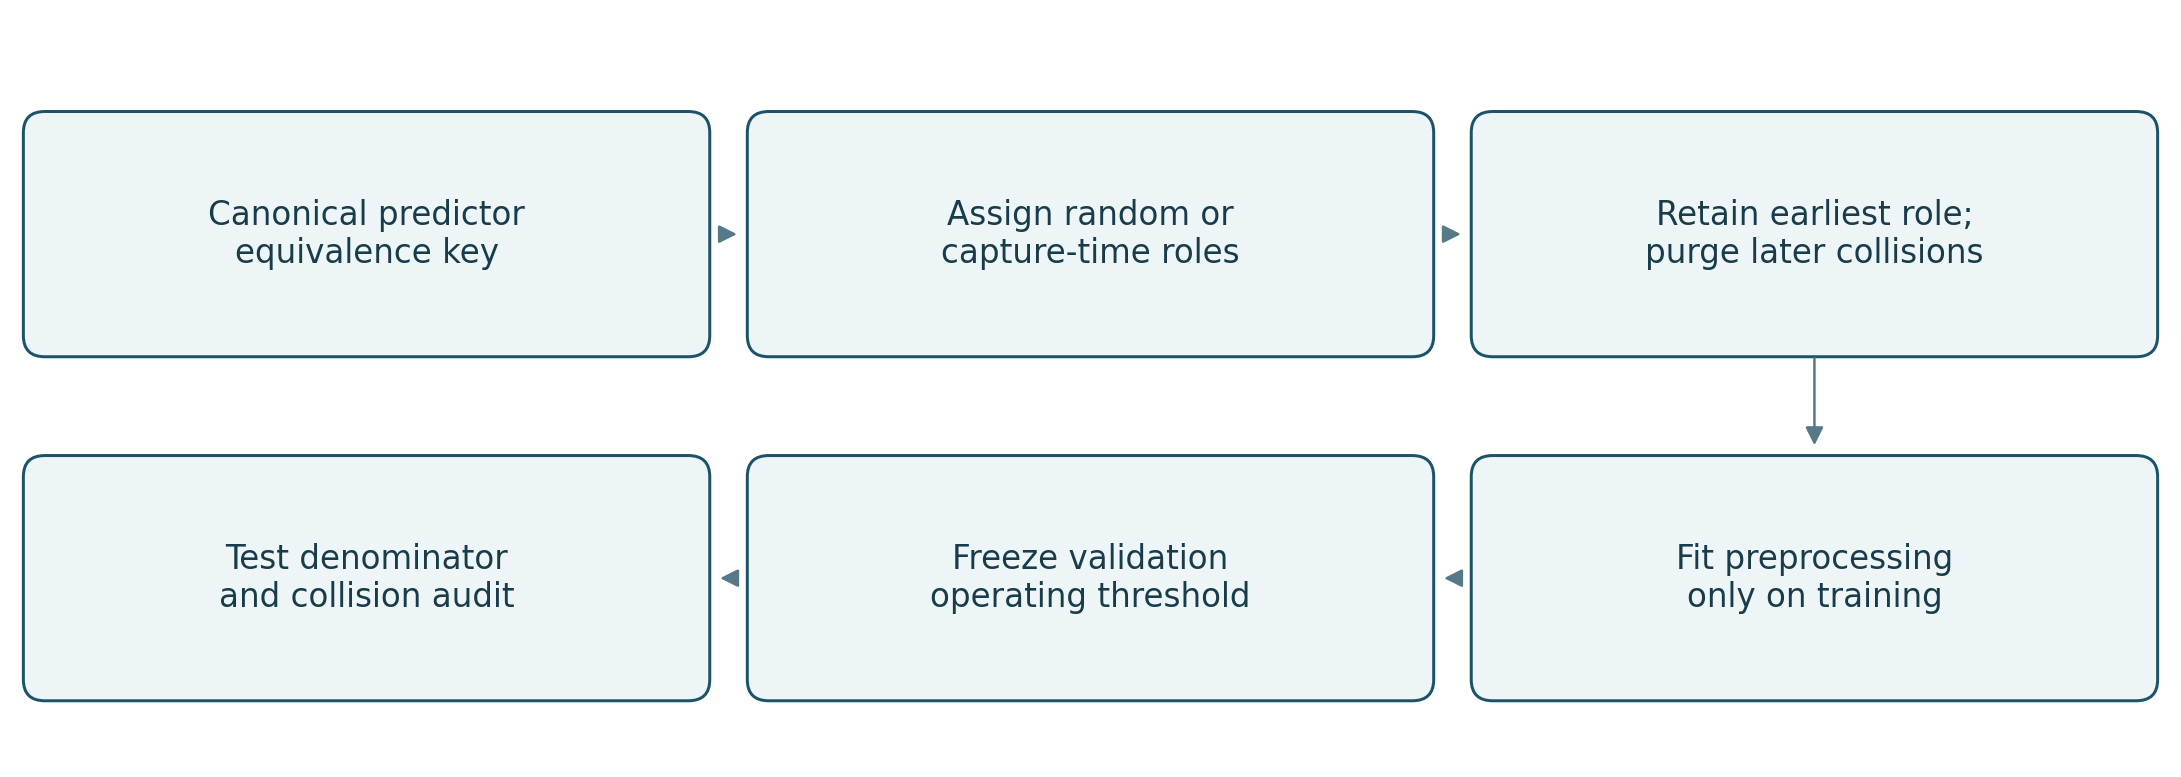
\includegraphics[width=\columnwidth]{../figures/leakage_splitting.png}\caption{Information boundaries for role assignment and evaluation. This conceptual diagram contains no performance measurements.}\label{fig:split}\end{figure}

\subsection{Feature and model identity}
A deployment contract includes feature names, ordering, admissible numerical domains and every fitted preprocessing parameter. Logistic regression requires its original coefficients and intercept; the random forest requires original split thresholds, topology and leaf distributions. K-Means requires training imputation, signed-log transformation, scaling and centers. Applying a convenient replacement transform would silently define a different model. Portable parameters are therefore verified against their archived source identities and independent Spark outputs before being accepted for interactive use.

Blank permitted inputs use training medians rather than statistics computed from a user's batch. Values outside the declared finite nonnegative range are diagnosed, and invalid rows remain distinguishable in exported results. This matters for reproducibility: silently dropping rows would change output counts, while silently coercing malformed values could create apparently valid predictions. The bounded upload interface is an engineering demonstration; it does not supply missing network context or validate measurements from arbitrary extractors.

\subsection{Fairness of the external comparison}
Column-name overlap is only a starting point for cross-dataset harmonization. Units, extraction windows, aggregation semantics and upstream filtering can differ. The three common features are explicitly conditional, and the external comparison excludes unsupported exact archived transfer. The source-only and target-trained models have different fitting populations and are reported separately. Neither the target chronological nor grouped result should be relabeled as source-only transfer.

Collision exclusions also affect the estimand. Excluding predictor collisions reduces a direct role-overlap route, but changes the retained population; it does not make two capture systems identical. The chronological and grouped test counts and exclusions are consequently preserved independently. Grouped hash sampling is approximately one seventh of the relevant population rather than an independent ten-percent sample within every role. Sample inclusion and cross-role purging are documented so that a reproduction does not silently create a different experiment.

\subsection{Operating budgets and adaptive selection}
A low false-positive budget constrains a detector's threshold on permitted validation data. It is not a guarantee that future benign captures have the same score distribution. The external source RF result illustrates the distinction: a threshold accepted under source validation can exceed that ceiling on a new source. Similarly, a high target ranking score can coexist with low calibrated recall when the selected budget requires a high threshold. Reporting a fixed 0.5 comparison is informative only when it is clearly separated from the predeclared calibrated result.

Adaptive policies add a second selection problem. A candidate must be trained on allowed released labels and accepted using the policy's history and budget, with activation restricted to a later prediction window. Reporting only the best candidate after observing all future errors would violate this ordering. Incumbent retention, cooldown and failed promotion are therefore part of the measured policy behavior. More candidate fitting is not intrinsically better when false positives, delayed labels or unstable calibration dominate the trade-off.

\subsection{Independent checks and scope accounting}
Numerical verification is layered. Source audits establish counts and eligibility; role receipts establish disjointness and purges; scoring receipts attach model and threshold identities; selected pattern rules are independently recounted; explanation receipts check reconstruction; and portable probes compare the implementation against Spark without retraining. These checks address different possible defects. Passing a portable parity check cannot repair poor temporal generalization, and passing a split check cannot establish external feature compatibility.

Experimental scope counts are likewise kept separate. Warm-up runs are not additional measured replicates. Synthetic policy configurations are not independent historical populations. An exported subset is not the complete set mined by FP-growth. The final evidence matrix records accepted phase checkpoints, while the master table attaches metric selectors and source hashes to key claims. This permits a reviewer to assess both a numerical assertion and the population to which it applies without relying on an unqualified dashboard headline.

\begin{figure}[t]\centering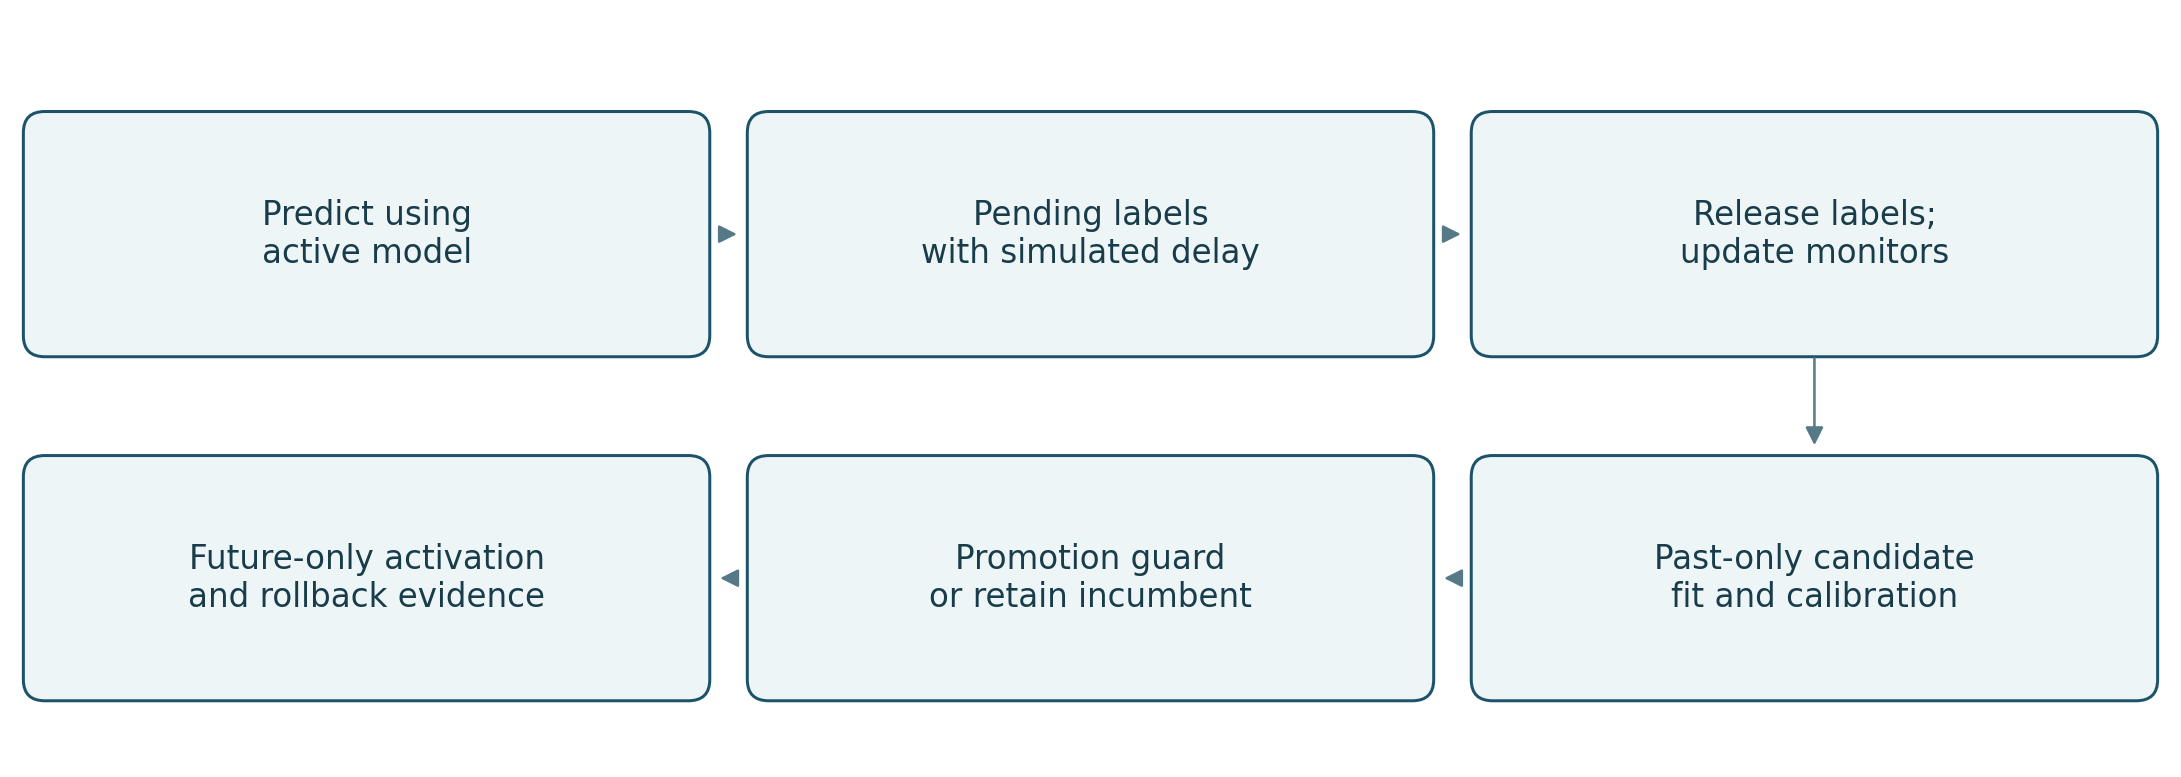
\includegraphics[width=\columnwidth]{../figures/adaptive_lifecycle.png}\caption{Future-only adaptive lifecycle. Labels are simulated as available according to the archived protocol; historical predictions are never revised by later candidates.}\label{fig:adaptive}\end{figure}

\section{Results}
\subsection{Leakage-aware generalization}
The random-forest group-sample baseline achieves attack recall 0.828169 on protocol A. Chronological B recall is approximately 0.0020 and unseen-family C recall approximately 0.0243. These are different test populations and should not be averaged into a single headline score. The A result supports a within-design discrimination claim, while the B and C results reveal a major generalization limitation. Randomly grouped performance is therefore insufficient evidence for future deployment.

The hybrid study combines calibrated supervised and novelty routes but does not consistently dominate all baselines. The selected B OR-fusion policy has zero attack recall at its archived operating point, despite a very small false-positive rate. This is a negative result, not a missing positive result to be replaced by post-hoc threshold selection. Family-stage diagnostics are conditional on binary routing: a correct family classifier cannot recover an attack already rejected by the binary detector. Research-only multiclass and hybrid components are consequently excluded from the portable dashboard's supported inference list.

\subsection{Frequent patterns and drift}
At minimum supports 0.10, 0.05, 0.02 and 0.01, the full-source FP-growth runs produce respectively 203, 298, 539 and 759 itemsets and 468, 629, 1,009 and 1,428 rules. The primary export retains 500 of 629 rules under the declared export bound; 20 selected rules receive independent count checks. Lower support increases the output search space, rather than proving more security-relevant knowledge. Rule interpretation remains descriptive and subject to the feature binning and capture mix.

ADWIN detects 24 of 27 targeted controlled episodes with zero stationary alarms across 11,520 eligible checks. Page--Hinkley detects 18/27 and KSWIN 17/27 with seven stationary false alarms. DDM's 6/6 result belongs to a distinct error-stream target set and cannot be ranked directly against the 27-episode feature-stream results. Historical analysis supports 45 of 49 windows; historical concept-drift ground truth is absent. Thus controlled detection sensitivity and retrospective capture shifts answer different questions.

\subsection{Adaptive learning and explanations}
On the primary 1,997,636-row adaptive evaluation, frozen P0 records 463 true positives and 4,691 false positives, approximately 0.00183 recall and 0.00269 FPR. P2 increases true positives to 634 but false positives to 9,835, approximately 0.00250 recall and 0.00564 FPR. P6 retains its incumbent and matches P0. These outcomes show a limited recall gain with a material false-positive trade-off, not unconditional adaptation success. The broader archive includes 288 synthetic experiments and 33 unique historical pipelines; these scope counts do not constitute 321 independent prospective trials.

Exact linear SHAP is reconstructed in log-odds across 48 variants. For the supported linear contract, the sum of base value and feature contributions reproduces the modeled output in its declared link space. It does not establish causal importance, and log-odds contributions must not be displayed as additive probabilities. Direct interventional tree SHAP for the archived PySpark trees remains unsupported. The accepted interface therefore exposes validated linear explanations and explicit unavailability rather than a fabricated tree explanation.

\subsection{Conditional external validation}
The CICIDS2017 mirror has eight CSV files totaling 884,645,759 bytes at pinned version 1. After eligibility rules, it supplies 2,830,743 rows: 2,273,097 benign and 557,646 attack. The chronological test has 308,939 rows, of which 129,275 are attacks and 179,664 benign. Collision exclusions number 287,528 in this protocol; the distinct grouped test contains 508,641 rows with 218,235 exclusions. These populations must not be combined. Exact upstream extractor builds and official-archive byte identity remain unverified.

Table~\ref{tab:external} reports primary chronological decisions. The source common-feature LR detects no attacks; source RF transfers some ranking signal but its source-validation operating threshold incurs a 4.254\% external benign FPR. A target-trained chronological RF achieves 5.436\% recall at its calibrated low-FPR threshold. Its fixed 0.5 threshold instead achieves 64.954\% recall and 1.722\% FPR. That contrast demonstrates threshold sensitivity, not permission to choose whichever test threshold looks best. The common-feature source models are newly trained three-feature baselines, not the exact archived 18-feature models.

\begin{table}[t]\caption{Primary external chronological test: 129,275 attacks and 179,664 benign rows. Validation-calibrated thresholds.}\label{tab:external}\centering\small
\begin{tabular}{lrrrr}\toprule Model & TP & FP & Recall & FPR\\\midrule Source LR &0&0&0&0\\Source RF&14,459&7,643&.11185&.04254\\Target LR&0&229&0&.00127\\Target RF&7,028&70&.05436&.00039\\\bottomrule\end{tabular}\end{table}

\subsection{Measured execution and usable inference}
Volume and worker experiments contain 48 measured and 16 warm-up runs, using actual populations 1,000,860, 3,998,178, 7,998,515 and 16,232,943. A four-worker setting is not consistently faster. The full-volume three-worker transform median is 21.076 seconds. These local-thread observations cannot establish multi-node scaling efficiency, resilience or production throughput.

In the matched one-million-row comparison, median end-to-end Pandas time is 0.242245 seconds and Spark 0.616481 seconds. Spark is therefore slower for this measured small workload, despite its broader distributed capabilities. Storage and workload consumption matter: the recorded full numeric Parquet artifact is 116,203,334 bytes with a 0.626799-second read median, versus 217,833,168-byte CSV and 1.921769 seconds. Different actions, caching and parsing costs must not be silently combined into a universal speedup.

The final advanced dashboard exposes 13 modules over nine navigation areas, 203 evidence tables and three portable models: LR, RF and K-Means. Its accepted 2,445-probe parity suite contains 100 LR, 2,245 RF and 100 K-Means probes. Maximum LR/RF probability deviations are approximately $1.53\times10^{-16}$ and $1.11\times10^{-16}$; maximum K-Means distance deviation is $4.37\times10^{-11}$. This establishes fidelity of bounded reconstruction, not additional predictive validity. Uploads are limited to 1 MiB and 500 rows, use the exact ordered feature schema, and retain invalid-row diagnostics. Manual and uploaded values use training medians; no transform is refitted on user input.

\section{Discussion}
The completed project demonstrates that large-scale cyberattack research can be made reproducible without hiding weak or negative results. Its most consequential findings are the collapse of some chronological operating points, the mixed value of fusion and adaptation, the difficulty of defensible feature transfer and the workload dependence of computational performance.

The final application computes genuine archived-model predictions and supported explanations while retaining source identities and bounds. Its usability and numerical compatibility are verified separately from detection quality. The final academic package closes the engineering and reporting workflow; it does not convert retrospective evidence into a claim of production readiness.

Future research could authenticate upstream extractor revisions, obtain prospective captures with legitimate ground truth, evaluate a prespecified common-feature transfer model on new untouched data and study calibrated operating policies under realistic analyst costs. Any new model selection would need fresh protocols and independent cohorts.

Engineering extensions could add a separately authorized hosted service, stronger access controls and tenant isolation, carefully monitored model lifecycle management and genuine multi-node benchmarks. These are proposals only. They are not implemented Phase 17 work or evidence already established by this submission.

\section{Threats to Validity}
The source mirror's upstream description and extraction revision are incomplete. The external mirror has explicit institutional provenance but no independently authenticated official-byte chain. Both are historical laboratory releases with capture-specific compositions. Exact cross-dataset event identity is not established, and common-vector collisions are not proof of duplicate events.

Repeated flows, finite capture days, group-aware sampling, approximate binned AUC, retrospective label release and bounded enriched cases limit statistical interpretation. Flow rows are not independent replications. Descriptive seed/repetition/capture-deletion ranges are not universal confidence guarantees. The secondary grouped target training budget is larger than an independent 10\%within-role sample because it shares a keyed hash with role assignment.

Direct interventional tree SHAP and original 18-feature external transfer remain unsupported. Novelty is not probability; association is not causation; historical replay is not live monitoring. Single-machine SparkContexts can share a warmed JVM and uncontrolled filesystem cache. Sampled RSS can miss transients, and Pandas process-tree memory can include a resident Spark JVM. Public deployment, authentication/tenant hardening and prospective operational validation remain future work.

\subsection{Reproducibility and evidence boundaries}
The evidence matrix links each completed research phase to a full Git checkpoint and report hash. The master results table adds exact row selectors and metric denominators. Compact aggregate outputs and portable parameters are versioned, while raw private inputs and credentials are excluded. The final academic package provides editable sources, diagrams, presentation, viva preparation and file hashes; recomputing private Spark experiments requires separately authorized source access and pinned runtime components.

There is no claim that these artifacts constitute an independently replicated clinical, operational or prospective security trial. Repeated runs estimate execution variability within the measured environment, not independent dataset uncertainty. Capture dependence, mirror provenance, sparse family distributions, binning choices, label delays and threshold-selection rules all limit extrapolation. A public dashboard deployment would be a separate administrative action, not evidence that the detector is safe for live automated response.

\section{Conclusion}
This case study shows why leakage controls, temporal roles, label availability and threshold decisions must accompany model scores. Grouped-random detection can coexist with poor chronological recall; associations and controlled drift alarms do not establish historical causal changes; and adaptation may buy small recall gains at substantial false-positive cost. Conditional external validation and matched local execution measurements expose further limits rather than erasing them. The defensible contribution is a traceable integrated evaluation and faithful inference demonstration. Future work requires stronger compatible provenance, prospective labels, independently calibrated operating budgets and multi-node measurements before broader effectiveness claims are justified.
\bibliographystyle{ieeetr}\bibliography{references}
\end{document}
